\begin{surferPage}[A3+- Singularity]{An $A_3^{+-}$ Singularity}
An $A_3^{+-}$ Singularity looks similar to a cusp of the form $A_2^{+-}$
    with equation $x^3+y^2-z^2$ except that it is also symmetric to $yz$--plane: 
    \[x^4+y^2-z^2=0.\]
    The equation is thus symmetric to all three coordinate planes which one
    can see by looking at the equation:
    \[(-x)^4+y^2-z^2=x^4+y^2-z^2.\] 
    Analogously, $y\mapsto -y$ and $z\mapsto -z$ do not have any effect.

    Similar to the cusp in the coffee cup we may see an $A_3^{+-}$ singularity
    when sunlight passes through a tee glass:
    \vspace*{-0.5em}
    \begin{center}
      \begin{tabular}{c@{\qquad}c}
        \begin{tabular}{@{}c@{}}
          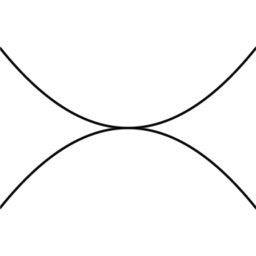
\includegraphics[width=1.4cm]{../../common/images/A3pm_cut_rot}
        \end{tabular}
        &
        \begin{tabular}{@{}c@{}}
          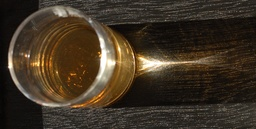
\includegraphics[height=1.4cm]{../../common/images/teeglas_detail}
        \end{tabular}
      \end{tabular}
    \end{center}
    \vspace*{-0.4em}
    The deformation into two double cone singularities (which exists according
    to the explanation to the $A_2^{+-}$ singularity) looks as follows:
%    \dontshow{
    % 
    \begin{center} 
      \vspace{-0.0cm}
      \begin{tabular}{@{}c@{\quad}c@{\quad}c@{}}
        \begin{tabular}{@{}c@{}}
          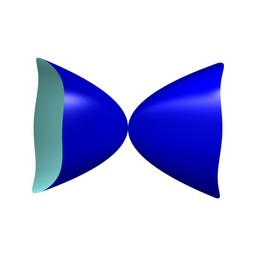
\includegraphics[width=1.2cm]{../../common/images/A3pm_0}
        \end{tabular}
        &
        \begin{tabular}{@{}c@{}}
          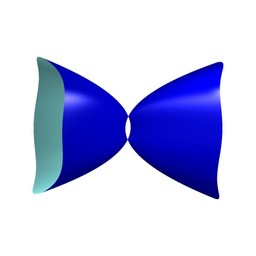
\includegraphics[width=1.2cm]{../../common/images/A3pm_1}
        \end{tabular}
        &
        \begin{tabular}{@{}c@{}}
          
\includegraphics[width=1.2cm]{../../common/images/A3pm_2}
        \end{tabular}
      \end{tabular}
    \end{center}
%    }
 
\end{surferPage}
